\documentclass{article}

%encoding
%--------------------------------------
\usepackage[utf8]{inputenc}
\usepackage[T1]{fontenc}
%----------------------------

%fonts
%--------------------------------------
%---------------
% \setromanfont{Times New Roman}
% \setsansfont{Arial}
% \setmonofont[Color={0019D4}]{Courier New}
%
\usepackage{libertine}
\usepackage{beramono}

%units
%--------------------------------------
\usepackage{siunitx}

%drawing
%------------------------------------
\usepackage{tikz} % To generate the plot from csv
\usepackage{pgfplots}
\usepackage{pgfplotstable}

\sisetup{
  round-mode          = places,
  round-precision     = 2,
}

\begin{document}

\begin{figure}
  \begin{center}

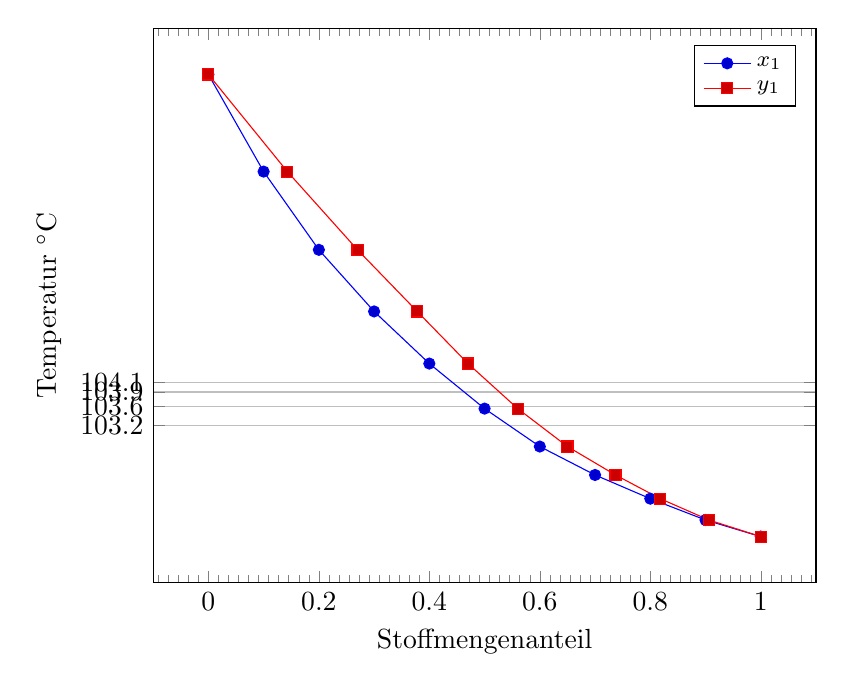
\begin{tikzpicture}
    \pgfplotsset{width=10cm,
        compat=1.3,
        legend style={font=\footnotesize}}
    \begin{axis}[
    xlabel={Stoffmengenanteil},
    ylabel={Temperatur \si\celsius},
    ytick={104.1, 103.9, 103.6, 103.2},
   minor tick num=10,
    ymajorgrids=true,
    legend cell align=left,
    legend pos=north east]
    \addplot table{
         0.00 110.60    
         0.10 108.55    
         0.20 106.90    
         0.30 105.60    
         0.40 104.50 
         0.50 103.55    
         0.60 102.75    
         0.70 102.15
         0.80 101.65    
         0.90 101.20
         1.00 100.85
    };
  \addplot table{ 
         0.000 110.60
         0.143 108.55
         0.270 106.90
         0.378 105.60
         0.470 104.50
         0.560 103.55
         0.650 102.75
         0.737 102.15
         0.818 101.65
         0.906 101.20
         1.000 100.85
};


    \addlegendentry{$x_1$}
    \addlegendentry{$y_1$}

     \end{axis}

    \end{tikzpicture}
\end{center}
\caption{Siedediagramm}
\end{figure}
\end{document}